

\documentclass{sig-alternate}
\pdfpagewidth=8.5in
\pdfpageheight=11in
\pgfplotsset{compat=1.10}

\begin{document}

\title{DEBS Grand Challenge: Real time Load Prediction and Outliers Detection using STORM  \titlenote{This work was financially supported by the Singapore National Research Foundation under its Campus for Research Excellence And Technological Enterprise (CREATE) programme.}}

\conferenceinfo{DEBS'14,} {May 26-29, 2014, MUMBAI, India.}
\copyrightetc{Copyright 2014 ACM \the\acmcopyr}
\crdata{978-1-4503-2737-4/14/05\ ...\$15.00.\\
http://dx.doi.org/10.1145/2611286.2611327} 

\clubpenalty=10000


\widowpenalty = 10000
\raggedbottom
\showboxdepth=5
\showboxbreadth=5

\numberofauthors{3} 
%
\author{
% You can go ahead and credit any number of authors here,
% e.g. one 'row of three' or two rows (consisting of one row of three
% and a second row of one, two or three).
%
% The command \alignauthor (no curly braces needed) should
% precede each author name, affiliation/snail-mail address and
% e-mail address. Additionally, tag each line of
% affiliation/address with \affaddr, and tag the
% e-mail address with \email.
%
% 1st. author
\alignauthor
      Abhinav Sunderrajan\\
             \affaddr{TUM CREATE Limited}\\
             \affaddr{1 CREATE Way}\\
             \affaddr{\#10-02 CREATE Tower}\\
             \affaddr{Singapore 138602}\\
             \email{abhinav.sunderrajan\linebreak @tum-create.edu.sg}
% 2nd. author
\alignauthor
Heiko Aydt\\
      \affaddr{TUM CREATE Limited}\\
	 \affaddr{1 CREATE Way}\\
	 \affaddr{\#10-02 CREATE Tower}\\
	 \affaddr{Singapore 138602}\\
     \email{heiko.aydt@tum-create.edu.sg}
% 3rd. author
\alignauthor
     Alois Knoll\\
           \affaddr{TUM CREATE Limited}\\
     	 \affaddr{1 CREATE Way}\\
     	 \affaddr{\#10-02 CREATE Tower}\\
     	 \affaddr{Singapore 138602}\\
          \email{knoll@in.tum.de}
}

\date{07 March 2014}
\maketitle
\begin{abstract}
In this work we present our solution towards the DEBS 2014 Grand challenge. We also discuss the set of novel and generic techniques used to enhance the performance of our STORM~\cite{storm} based stream-processing platform while implementing the challenge queries.
\end{abstract}

% A category with the (minimum) three required fields
\category{H.4}{Information Systems Applications}{General}
\keywords{Stream processing engine, Complex event processing, Stream archive queries} % NOT required for Proceedings

\section{INTRODUCTION}
\label{sec:introduction}

The DEBS Grand Challenge 2014 provided recordings \linebreak from smart plugs measuring power consumption related values which are deployed across a number of households~\cite{ziekow2014challenge}. The goal of the challenge is to develop a stream-processing system for computing short term load-predictions and detecting outliers over this high velocity data stream. We made use of an open-source distributed stream processing system called STORM for horizontally scaling our solution. We employ generic techniques such as archive data streams, hybrid queries and a novel architecture which combines a high-level CEP system with STORM for better performance.

 The organization of the paper is as follows. In Section ~\ref{sec:queries} we discuss the two queries comprising the challenge. In Section \ref{sec:architecture} we discuss the architecture and elaborate upon the optimizations incorporated to enhance the performance of our stream-processing system. Section \ref{sec:evaluation} evaluates the system while executing the challenge queries. The paper concludes in Section \ref{sec:conclusion}.

\section{QUERIES}
\label{sec:queries}

\subsection{Query 1}
\label{sub:query 1}
Query 1 involves predicting short term load over time intervals ranging from 1 minute to 60 minutes at the resolutions of individual houses and plugs. The prediction model though conceptually simple is more of a query processing problem. The predicted load is the average of current load (averaged over a time interval) and the median load for the past 'N' days at the time slice  corresponding to the prediction interval. We employ {\it proactive archive streams} discussed in Section \ref{sub:proarchstreams} for efficient retrieval of specific data from a massive archive consisting of historic load values. 


\subsection{Query 2}
\label{sub:query 2}
Query 2 involves estimating the outliers in terms of load consumption by computing the percentage of plugs in each house having a median load greater than the global median load for all plugs  over a specified time interval. The primary issue involved in implementing a solution for this query is the process of computing the global median load over the past 1 hour and the past 24 hours by using a sliding window with a slide equal to 1 second. The naive approach of storing the load values for each reading over a high volume data stream over long periods of time is  infeasible. The operation of computing global median for all plugs is further complicated by the fact that the operation cannot parallelized making it non-scalable. 

\section{ARCHITECTURE \& OPTIMIZATIONS}
\label{sec:architecture}
In this section we describe the architecture of our data-stream processing platform which is implemented in Java. We also discuss the optimizations incorporated to increase the performance and scalability of our system.

\subsection{Core components}

\subsubsection{STORM}
\label{subsub:storm}
The data stream processing platform has been built using {\it STORM} as the core framework. STORM is an open-source distributed real time computation engine which enables a developer to neatly package the stream-processing logic to processing units called {\it bolts}. Each bolt can be parallelized by configuring the number of threads it needs to execute. STORM also defines an abstraction called the {\it spout} which is the source of input data-streams.

 A STORM {\it topology} represents a network of spouts and bolts with each bolt subscribing to the output of a spout or a preceding bolt. The entire topology can be distributed across a cluster of slave nodes making it scalable. Further, STORM uses a lock-free ring buffer called the {\it LMAX disruptor}~\cite{lmax} for efficient data transfer between the bolts. We have leveraged the power of LMAX disruptor in intra bolt threads for efficiency and to mitigate the effects of {\it stop-the-world generational garbage collection}~\cite{sun}.


\subsubsection{Redis}
\label{sub:redis}
The need for a centralized in-memory data-structure was necessitated due to the distributed nature of the  stream-processing system where the processing bolts could reside in any node in the cluster. {\it Redis}~\cite{redis} can be described an in-memory key-value database. Redis enables the storage of data-structures such as lists, Maps and Sets in memory allowing extremely fast retrieval of a value from these data-structures using an associated key.


\subsection{Optimizations}
\label{sec:optimizations}
In this subsection we discuss the optimizations made for enabling our stream-processing system to address the queries posed in the challenge. The techniques discussed are largely generic and can be adopted to enhance the performance and scalability for purposes other than this challenge.


\subsubsection{Esper-enriched bolts}
\label{sub:esper}
Despite STORM enabling the overlying stream processing platform to be truly scalable, it does provide semantics to define sliding windows. We have incorporated Esper~\cite{esper} in our system to create {\it Esper-enriched} bolts where sliding window and group operations were necessary. Esper is a high-level event-stream processing engine with Java and .NET bindings. 

Esper also provides a SQL-like language called {\it Esper processing language} (EPL) to perform operations such as select, project, filter and join on event streams. EPL  defines a variety of sliding and tumbling windows for computing aggregates. Each processing thread of an Esper-enriched bolt is associated with an unique {\it Esper-engine instance} to process the tuples using an Esper query.
 
\subsubsection{Proactive archive data-streaming}
\label{sub:proarchstreams}
Retrieving historic data from massive archives while processing high-velocity live streams is a challenge. Considering that queries to a massive archives are costly, intelligent techniques should be employed to avoid bottlenecks. For the grand challenge, we ensure that the archive data in appropriately sized chunks (which for Query 1 described in Section~\ref{sub:query 1} would equal the defined time slice) are fetched before the arrival of the live event (i.e. pro-actively) to minimize latency to a bare minimum. Considering an example where the archive load aggregates for the past 3 days are required, three concurrent database connections from Monday through Wednesday are used to stream per plug load aggregates between  00:45:00 hours and 01:00:00 hours. It is assumed that the current time is 00:15:00 hours on a Thursday. The per plug load aggregates for the aforementioned time interval are computed and sent to the platform through as many  {\it archive stream spouts} as the concurrent database connections. 

The load aggregates per plug (and per house) per time-slice interval are stored in a Redis data-structure. For minimal database-query latency the stream-archive table is indexed on time stamp. With knowledge on the approximate live-stream velocity and time-slice over which prediction is to be computed, the interval at which archive load aggregates are retrieved can be set to ensure that the values are stored in memory before the arrival of live-stream tuples. We refer to this technique as {\it proactive archive streaming} since only the relevant archive records are streamed and stored in memory for operations such as joining and comparison with the live-stream tuples prior to their arrival. The technique is based on the {\it porthole scan}  approach elaborated in~\cite{tufte2007travel}.

\section{Query topologies}
 
\subsection{Topology for Query 1}
\label{sub:q1-topology}

\begin{figure}[!htbp]
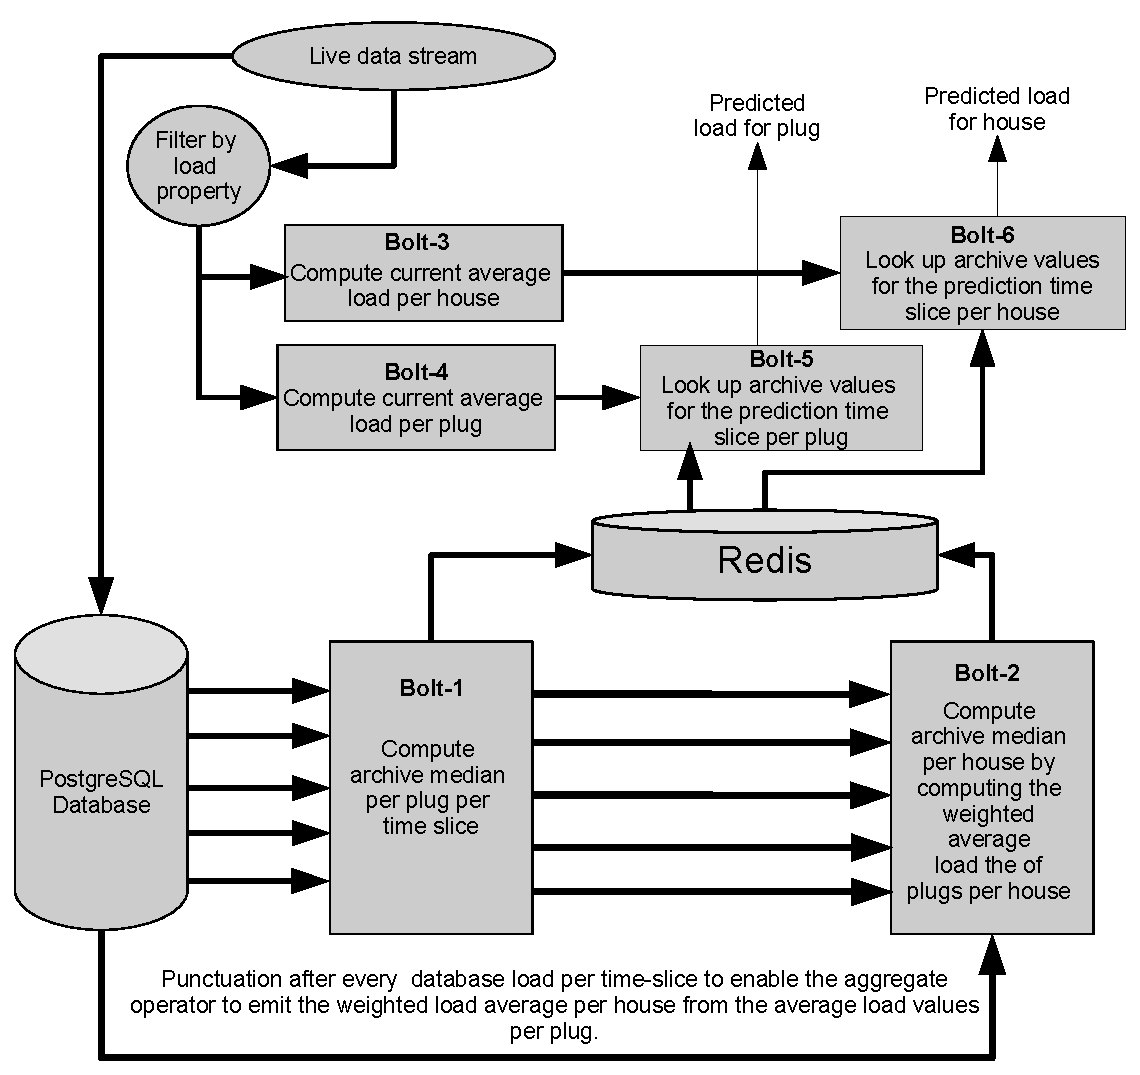
\includegraphics[scale=0.42]{query1.pdf}
\caption{STORM topology for query 1}
\label{fig:q1-topo}
\end{figure}

Figure~\ref{fig:q1-topo} shows the STORM topology for Query 1. The stream archive is stored in a PostgreSQL database. Concurrent database connections are setup to retrieve historic load aggregates per plug, per time interval through archive streams discussed in Section~\ref{sec:optimizations}. The retrieved values per plug. per time slice, per day are stored in a circular-buffer of size N. The size of the  buffer equals the  number of days in the archive which are required for load prediction. Storing the archive aggregates in a circular-buffer ensures that irrespective of the number of archive streams we begin with, the count reduces to one after 24 hours since the other N-1 values are already present. Bolt-1 shown in Figure~\ref{fig:q1-topo} is responsible for computing the per plug archive aggregates before storing the values to the corresponding circular buffer in Redis. Concurrently  Bolt-2 connected to  Bolt-1 computes the archive aggregates per house, per time slice, per day by grouping the tuples belonging to a single house and calculating the weighted-average before storing in Redis.

 Computing a weighted average is a blocking operation which is resolved by using {\it punctuations}~\cite{tucker2003exploiting}. Bolt-3 and Bolt-4 group the live stream tuples per house and per plug respectively to compute the current load average over the specified time-interval. Bolt-5 and Bolt-6 look up the Redis data-structure to retrieve the list storing the archive load aggregates for computing the archive-median load values for future load prediction.


\subsection{Topology for Query 2}
\label{sub:q2-topology}  
\begin{figure}[htbp]
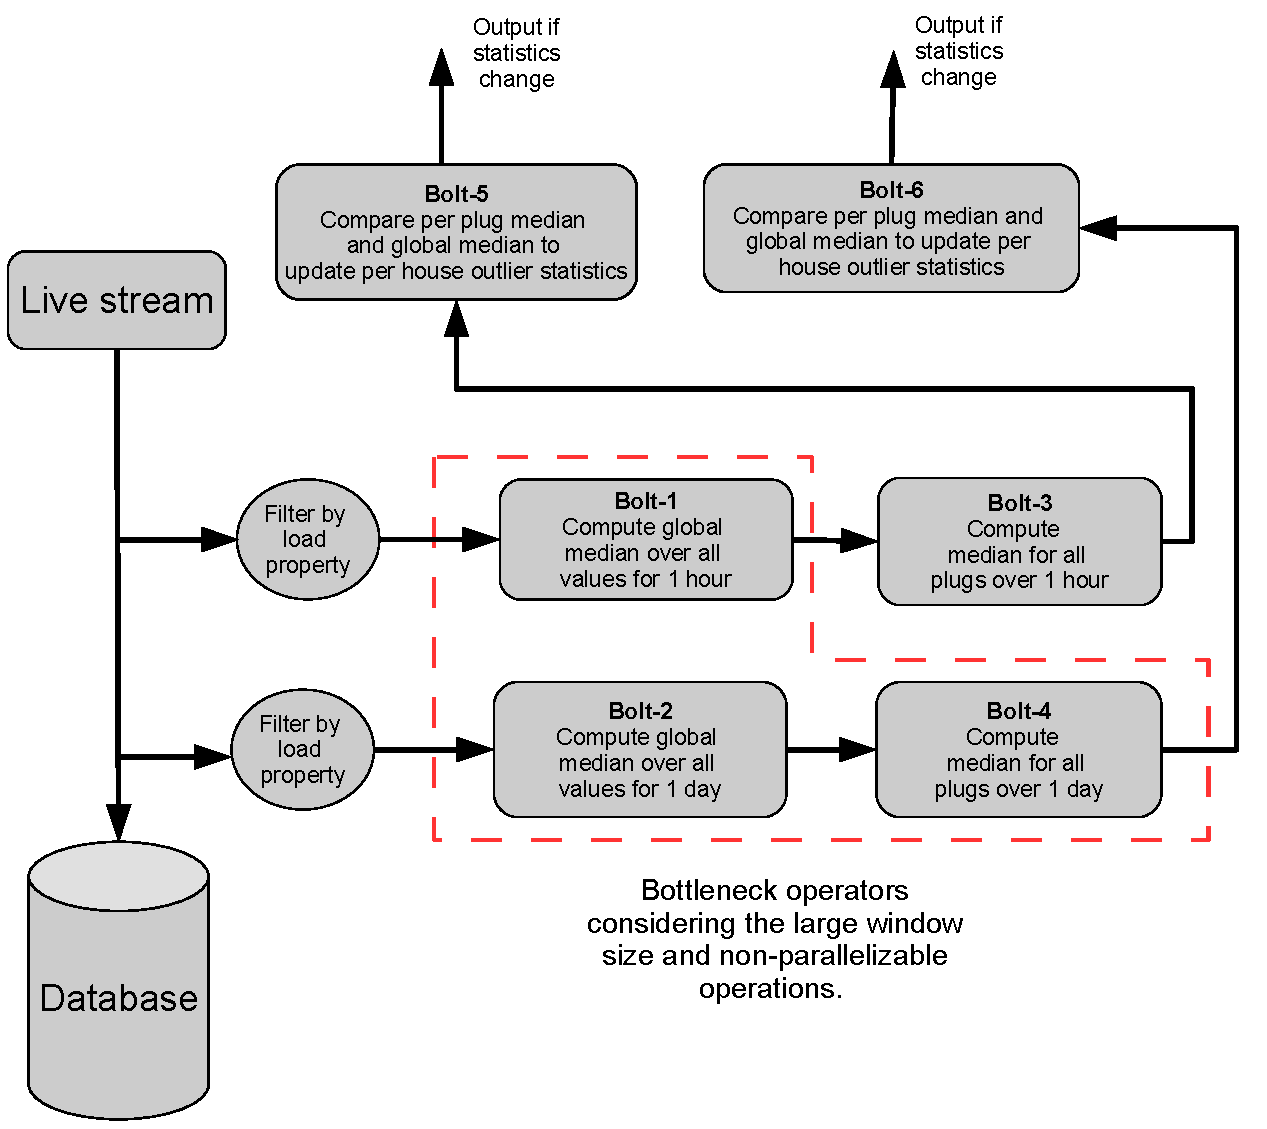
\includegraphics[scale=0.393]{query2.pdf}
\caption{STORM topology for query 2}
\label{fig:q2-topo}
\end{figure}

 Figure~\ref{fig:q2-topo} shows the STORM topology of Query 2. The operators for computing the global median over a sliding time windows of 60 minutes and 24 hours need to be optimized for reasons explained in Section~\ref{sub:query 2}.  As outlined, computing medians over huge sliding windows is challenging if exact results need to be produced. We thus employ stream sampling techniques to produce approximate median load over the data-stream. We thus decided to use the {\it priority-sample algorithm}~\cite{babcock2002sampling} which is specifically suitable for sampling over time-stamp based sliding windows. The solution though approximate is quite accurate considering that the individual load values are repetitive. Priority-sampling is also used to compute the global median over an hour and over a day. 
 
 Bolt-3 computing medians per plug over a sliding window of an hour computes the exact median while the bolt doing the same operation over one day uses priority-sampling. A Redis based in-memory data structure is updated when ever the percentage of outliers per house changes and the results are sent to the stream subscribers.
 


\section{EVALUATION}
\label{sec:evaluation}


In this section we evaluate the performance of our stream processing system under the purview of the challenge guidelines. The experiments were performed on an  HPC cluster with CentOS 6.4 operating system. The JVM memory allocated to each worker node and a single {\it nimbus} i.e. master node in the STORM cluster was restricted to 2 GB. The {\it parallelism} for all processing bolts (indicating the number of threads per bolt in a node) in the STORM topology was  constant throughout all evaluations and thus have no bearing on the relative results.

For workload evaluations, we did not split the input CSV file provided for the challenge into three separate files (as suggested in the challenge guidelines). Rather we added a filter at the live stream spout filtering on the house-id. Finally filtering for load/work and any other property such as house is performed at the stream processing system. Thus the parameter live-stream velocity always implies the number of events sent by the live data-streaming system to the stream-processing platform per second.

\subsection{Evaluation for Query 1}
\label{sub:eval-query 1}


For all readings shown below we have restricted the number of archive data streams to three. We have not considered an evaluation which varies the number of archive streams as it is out scope for this challenge. We refer to Query 1a as the query which predicts the load per house and Query 1b as the one which predicts the load per plug. Throughput refers to the number of tuples received by the stream subscriber per second.
% Please remember to add \use{multirow} to your document preamble in order to suppor multirow cells
\begin{table}[!htbp]
\centering
\begin{tabular}{|c|c|c|c|}
\hline
\begin{tabular}[c]{@{}c@{}}Number of \\slave nodes\end{tabular} & Query    & \begin{tabular}[c]{@{}c@{}}Average \\ latency \\ (ms)\end{tabular} & \begin{tabular}[c]{@{}c@{}}Average \\ throughput\end{tabular} \\ \hline
\multirow{2}{*}{1}                                                & Query 1a & 1071.55                                                             & 4301.55                                                        \\ \cline{2-4} 
                                                                  & Query 1b & 1375.245                                                             & 4392.25                                                        \\ \hline
\multirow{2}{*}{2}                                                & Query 1a & 458.92                                                             & 4907.40                                                       \\ \cline{2-4} 
                                                                  & Query 1b & 289.05                                                             & 4907.40                                                       \\ \hline
\multirow{2}{*}{3}                                                & Query 1a & 597.43                                                             & 5038.02                                                       \\ \cline{2-4} 
                                                                  & Query 1b & 499.01                                                             & 5086.04                                                       \\ \hline
\multirow{2}{*}{4}                                                & Query 1a & 802.65                                                             & 5156.86                                                       \\ \cline{2-4} 
                                                                  & Query 1b & 549.84                                                             & 5196.07                                                       \\ \hline
\end{tabular}
\caption{\label{table:q1-nodes} Query 1 parameters on varying the number of processing nodes}
\end{table}
 
 Table~\ref{table:q1-nodes} shows the result of varying the number of processing nodes while maintaining a constant workload of 40 houses and restricting  the live stream velocity to 10,000 messages per second. The minimum number of slave nodes required was found to be two. Lack of sufficient memory (fixed at 2 GB per node) and restricted parallelism per node was found to be the main bottleneck while processing the live tuples using a single slave node.
 
 
 
% Please add the following required packages to your document preamble:
% \usepackage{multirow}
\begin{table}[!htbp]
\begin{tabular}{|c|c|c|c|}
\hline
\begin{tabular}[c]{@{}c@{}}Time-slice\\ (minutes)\end{tabular} & Query    & \begin{tabular}[c]{@{}c@{}}Average \\ latency \\ (ms)\end{tabular} & \begin{tabular}[c]{@{}c@{}}Average \\ throughput\end{tabular} \\ \hline
\multirow{2}{*}{1 min}                                         & Query 1a & 423.24                                                             & 2520.83                                                       \\ \cline{2-4} 
                                                               & Query 1b & 328.34                                                             & 2520.83                                                       \\ \hline
\multirow{2}{*}{5 min}                                         & Query 1a & 521.51                                                             & 2520.83                                                       \\ \cline{2-4} 
                                                               & Query 1b & 305.57                                                             & 2520.83                                                       \\ \hline
\multirow{2}{*}{15 min}                                        & Query 1a & 510.47                                                             & 2525.21                                                       \\ \cline{2-4} 
                                                               & Query 1b & 293.52                                                             & 2525.21                                                       \\ \hline
\multirow{2}{*}{60 min}                                        & Query 1a & 547.60                                                             & 2511.15                                                       \\ \cline{2-4} 
                                                               & Query 1b & 361.10                                                             & 2507.97                                                       \\ \hline
\multirow{2}{*}{120 min}                                       & Query 1a & 510.62                                                             & 2512.87                                                       \\ \cline{2-4} 
                                                               & Query 1b & 378.78                                                             & 2512.87                                                       \\ \hline
\end{tabular}
 \caption{\label{table:q1-timeslice} Query 1 parameters on varying prediction time-interval.}
\end{table}
 

 

  % Please remember to add \use{multirow} to your document preamble in order to suppor multirow cells
 \begin{table}[h]
 \begin{tabular}{|c|c|c|c|}
 \hline
 \begin{tabular}[c]{@{}c@{}}Number\\ of houses\\ processed\end{tabular} & Query    & \begin{tabular}[c]{@{}c@{}}Average \\ latency \\ (ms)\end{tabular} & \begin{tabular}[c]{@{}c@{}}Average \\ throughput\end{tabular} \\ \hline
 \multirow{2}{*}{10}                                                    & Query 1a & 64.41                                                              & 1219.11                                                       \\ \cline{2-4} 
                                                                        & Query 1b & 4.69                                                               & 1215.10                                                       \\ \hline
 \multirow{2}{*}{20}                                                    & Query 1a & 67.44                                                              & 2224.08                                                       \\ \cline{2-4} 
                                                                        & Query 1b & 1.89                                                               & 2220.36                                                       \\ \hline
 \multirow{2}{*}{40}                                                    & Query 1a & 1071.55                                                            & 4301.55                                                       \\ \cline{2-4} 
                                                                        & Query 1b & 1375.245                                                           & 4392.25                                                       \\ \hline
 \end{tabular}
 \caption{\label{table:q1-workload} Query 1 parameters on varying workload}
 \end{table}
  
  Table~\ref{table:q1-timeslice} shows the results of varying the time slice over which future load was predicted. The workload, live stream velocity and the number of processing nodes were kept constant at 40 houses, 5000 messages per second and two respectively throughout this evaluation. The results indicate that the throughput and latency are time-slice invariant. The results are not surprising considering that the operator computing load averages does not store individual values and instead computes rolling-averages. 
  
  Finally  Table~\ref{table:q1-workload} shows the results of varying the workload while keeping the live-stream velocity (10,000 messages per second) and the number of processing nodes (one) constant. As expected the performance in terms of latency and throughput is best when the number of houses processed is decreased thus reducing the workload.


\subsection{Evaluation for Query 2}
\label{sub:eval-query 2}

For all evaluations of Query 2, the live-stream velocity was fixed at 10,000 messages per second. We refer to the query computing the outliers over a sliding window of 60 minutes as Query 2a and the  query computing outliers over a  24 hour sliding window as Query 2b. The throughput for Query 2 (both a and b) are not considered given that the output tuples are emitted only when the percentage of outliers in a house change.

The results of varying the number of processing nodes while keeping the workload constant (40 houses) are shown in Figure \ref{fig:q2-nodes}. The results indicate that a minimum of three  nodes were required for processing the workload. Figure \ref{fig:q2-workload} shows the results of varying workload while keeping the number of processing nodes constant at two.

\begin{figure}[!htbp]
\begin{tikzpicture}
\begin{axis}[
 width=0.4\textwidth,
 height=0.26\textwidth,
ybar,
    enlargelimits=0.15,
    legend style={at={(0.5,-0.19)},
      anchor=north,legend columns=-1},
    ylabel={\ Average latency(ms)},
    symbolic x coords={1 node,2 nodes,3 nodes,4 nodes},
    xtick=data,
    ]
\addplot [pattern=north west lines,pattern color= blue]
	coordinates {(1 node, 4323) (2 nodes, 3513)
		 (3 nodes,584.9) (4 nodes,603) };

\addplot [pattern=north east lines,pattern color= red]
	coordinates {(1 node,1913) (2 nodes,712) 
		(3 nodes,368) (4 nodes,393)};

\legend{Query 2a,Query 1b}
\end{axis}
\end{tikzpicture}
\caption{Query 2 parameters on varying the number of processed nodes.} \label{fig:q2-nodes} 
\end{figure}



\begin{figure}[h]
\begin{tikzpicture}
\begin{axis}[
 width=0.38\textwidth,
 height=0.26\textwidth,
ybar,
    enlargelimits=0.15,
    legend style={at={(0.5,-0.19)},
      anchor=north,legend columns=-1},
    ylabel={\ Average latency(ms)},
    symbolic x coords={10 houses,20 houses,40 houses},
    xtick=data,
    ]
\addplot [pattern=north west lines,pattern color= blue]
	coordinates {(10 houses, 148.8) (20 houses, 233.6)
		 (40 houses,3513.7) };

\addplot [pattern=north east lines,pattern color= red]
	coordinates {(10 houses,104.70) (20 houses,136.5) 
		(40 houses,712.05) };

\legend{Query 2a,Query 1b}
\end{axis}
\end{tikzpicture}
\caption{Query 2 parameters on varying workload.} \label{fig:q2-workload} 
\end{figure}





\section{CONCLUSIONS}
\label{sec:conclusion}

In this paper we presented a stream-processing system to address the queries posed by the DEBS grand challenge 2014. We made use of STORM to enhance the scalability of our platform. To minimize the latency associated with accessing a massive archive, we employed archive streams. Archive streams enabled us to fetch the historic data in chunks of optimal size pro-actively. Sliding window queries and grouping operations over the data-streams were implemented using Esper-enriched bolts. Experiments show that we were able to process data streams at velocities of 10,000 messages per second using just two processing nodes while keeping memory consumption to a reasonable 2GB per node.


%
% The following two commands are all you need in the
% initial runs of your .tex file to
% produce the bibliography for the citations in your paper.
\bibliographystyle{abbrv}
\bibliography{sigproc} 

\end{document}
